\documentclass[11pt]{article}
\usepackage[margin=0.88in]{geometry}
\usepackage{amsmath,booktabs,graphicx,array}
\usepackage[T1]{fontenc}
\usepackage{natbib}
\usepackage[hidelinks]{hyperref}
\title{From Actionless Robot Demonstrations to Policy Data:\ A Lift Pilot of Inverse Dynamics, Visual Descriptions, and Hosted Decision-Based Selection}
\author{Paul Ruiz Alliata}
\date{September 21, 2026}

\begin{document}
\maketitle

\begin{abstract}
We study whether a pretrained vision model helps turn robot demonstrations
whose actions are hidden from the learning pipeline into useful policy data.
In a robomimic Lift pilot, 24 action-labeled demonstrations train local
inverse-dynamics and grounding models; 16 further training demonstrations
provide observations for pseudo-labeling. A policy trained on 24 gold
demonstrations succeeds on 14.7\% of closed-loop trials. Adding 16 local
inverse-dynamics pseudo-labeled demonstrations yields 32.7\%; adding 16
Gemini 3.6 Flash semantic descriptions grounded into actions yields 34.0\%.
The prespecified visual-versus-inverse comparison is +1.3 percentage points
(original paired-start 95\% interval $[-9.3,+11.3]$), which does not establish
an advantage. Filtering eight pseudo-labeled demonstrations yields 42.0\%
for the inverse model and 46.7\% for a local inverse-plus-visual hybrid;
the latter difference is uncertain across three training seeds. In a later
follow-up, hosted TypeSafe Jev 1.13 judged the \emph{cached text descriptions}
to select eight of the same hybrid pseudo-labeled demonstrations. This policy
reached 38.7\%, versus 42.0\% when selection used Gemini's confidence and
46.7\% with the existing hybrid risk score. Hosted Jev's held-out error-risk
ranking was near chance (AUC 0.491). These are small, single-task pilots with
no locked-test evaluation. They support the utility of pseudo-labeled data
but do not establish added value from the visual or hosted decision layers
over the corresponding local controls.
\end{abstract}

\section{Question and scope}
Action-conditioned robot training needs pairs of observations and executable
controls. Videos and state trajectories often lack accessible action labels.
The motivating Jev concept proposes an auditable data layer that infers useful
transition descriptions or action distributions, then exports trajectories
for downstream training. This study tests a limited part of that proposal:
whether pseudo-actions inferred from one simulated manipulation task improve
an independently trained behavior-cloning (BC) policy. No action-conditioned
world model was trained or evaluated here. The raw robomimic files contain
actions for all demonstrations; the experimental software masks the actions
of the 16 pseudo-label targets. This is a controlled missing-label simulation,
not a collection of naturally actionless videos.

The study has three distinct components. A trained inverse-dynamics model
(IDM, arm B2) predicts native actions from frozen DINOv2 visual features.
Gemini 3.6 Flash reads rendered RGB frames and returns a 24-dimensional
semantic description; a trained grounding network maps that description and
current features into native actions. An inverse-dynamics/semantic hybrid
combines B2 predictions with the Gemini descriptions. TypeSafe Jev 1.13,
accessed through OpenRouter, accepts text or JSON and returns typed decisions,
not images or continuous robot actions \citep{typesafe,openrouter}. It was
first used in the later E3b data-selection follow-up. Historical experiment
IDs containing ``JV'' denote the Gemini-grounded or hybrid architecture;
they do not indicate a TypeSafe Jev call.

\section{Data, models, and evaluation}
\paragraph{Data and controller.} The Lift dataset has 200 episodes. A fixed
split reserves 120 for training, 20 for development, 20 for calibration, and
40 for a locked test. The pilot uses the first 40 training episodes: 24 with
visible actions for annotator and policy training, plus 16 whose action arrays
are hidden from pseudo-label generation. Eight development episodes inform
selection, eight calibration episodes fit risk maps, and 12 other development
episodes form an evaluation holdout. The 40-episode test remains untouched.
The 7-dimensional OSC\_POSE controls are bounded in $[-1,1]$, with a binary
gripper channel; the recorded controller runs at 20 Hz. Grounding models
receive only the 24 training action labels. The 40-gold policy reference also
uses the native actions of the 16 otherwise masked training episodes and
therefore has a larger label budget.

\paragraph{Pseudo-action generation.} Local B2 predicts an action
distribution from DINOv2 features of short observed transitions. Local B3 is
a feature-difference reconstruction comparator; no B3 policy was retrained
in E3. The Gemini semantic path sends four $256\times256$ agent-view images
around each transition to \texttt{google/gemini-3.6-flash}, encodes its fixed
JSON response as a 24-dimensional vector, and trains a small local grounding
network on 24 gold episodes. A separate direct-output query asks Gemini for
seven native-action values and supplies three fixed examples from the same
label budget; this is a reconstruction diagnostic, not a policy arm. The
hybrid grounding network takes B2 outputs, Gemini semantics, and visual
features. Grounding, risk fitting, and policy training are distinct stages.

\paragraph{Risk and policy protocol.} An action is marked bad when its mean
position error exceeds the development-set B2 median threshold, its mean
rotation error exceeds the corresponding threshold, or its gripper sign is
wrong. The thresholds are 0.1168 and 0.0242 in native action units. Each
method's uncertainty score is mapped to empirical error on the eight
calibration episodes with isotonic regression. Filtering ranks the 16
unlabeled \emph{episodes} by mean predicted risk and keeps eight; it does not
discard individual transitions. Each policy has a 19-dimensional low-level
observation input, a two-layer 256-unit BC network, and 3,000 optimizer
updates. Three independently initialized policies per arm run on the same 50
simulator starts (seeds 10000--10049), for 150 closed-loop trials per arm and
a 200-step horizon. The success metric is Lift's simulator success check.
Policy seeds, not rollouts, are the limited training replication.

\paragraph{Later hosted decision experiment.} E3b was specified \emph{after}
E3 outcomes were known. It sent existing Gemini semantic JSON, not images or
native labels, to \texttt{typesafe/jev-1.13}. Three fixed Noul questions
judged motion ambiguity, contact ambiguity, and internal inconsistency.
The largest returned probability served as an uncalibrated uncertainty
score; a new isotonic map was fitted on 383 calibration transitions. A
matched control used $1-\text{Gemini confidence}$ with the same calibration
code. Each method kept eight of the same 16 episodes. Both E3b policies
reused the \emph{same saved hybrid pseudo-action arrays}, the same 24 gold
episodes, policy settings, and paired evaluation starts. The original
hybrid-risk filter is a historical comparator with a different existing
calibration implementation. Exact repeated semantic inputs were cached, so
1,646 scored transitions required only 72 distinct hosted requests.

\section{Closed-loop policy results}
Table~\ref{tab:policy} and Fig.~\ref{fig:policy} report all evaluated
policy arms. P0, B2, and the 40-gold reference anchor the interpretation.
The unfiltered Gemini-grounded arm exceeded P0 by 19.3 percentage points,
but only by 1.3 points over B2. The latter interval includes substantial
benefit and harm; it is not an equivalence test. The unfiltered hybrid was
below B2. The filtered Gemini-grounded arm also fell to 26.0\%, a result
that the original manuscript omitted from its overall conclusion.

\begin{table}[t]
\centering\small
\caption{Lift policy success. Every row except the 40-gold reference uses
24 gold demonstrations. ``All'' means 16 pseudo-labeled demonstrations;
``filtered'' means eight. Each mean covers three policy seeds and 50 shared
starts per seed. E3b rows reuse E3 hybrid pseudo-actions and vary only the
episode selector.}
\label{tab:policy}
\begin{tabular}{p{0.62\linewidth}r}
\toprule
Policy data and selector & Mean success \\
\midrule
P0: 24 gold only & 14.7\% \\
Local B2: all 16 pseudo-labeled & 32.7\% \\
Local B2: filtered eight & 42.0\% \\
Gemini semantics + local grounding: all 16 & 34.0\% \\
Gemini semantics + local grounding: filtered eight & 26.0\% \\
Local B2 + Gemini hybrid: all 16 & 24.0\% \\
Local hybrid: existing risk filter & 46.7\% \\
Same saved hybrid actions: Gemini-confidence filter (E3b) & 42.0\% \\
Same saved hybrid actions: hosted TypeSafe Jev filter (E3b) & 38.7\% \\
P-REF: 40 gold demonstrations & 45.3\% \\
\bottomrule
\end{tabular}
\end{table}

\begin{figure}[t]
\centering
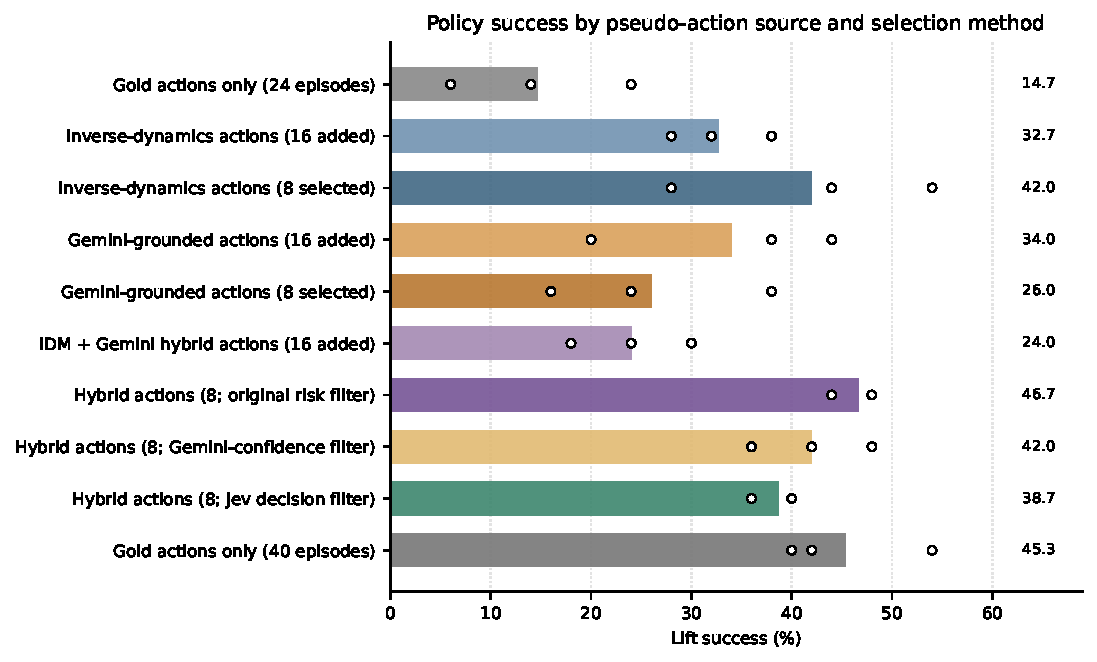
\includegraphics[width=\linewidth]{figs/policy_results.pdf}
\caption{All policy arms. Every pseudo-action row adds the indicated episodes
to the same 24 gold episodes. The Jev row uses Jev only to select episodes;
its actions come from the saved inverse-dynamics/Gemini hybrid. White points
show the three training-seed success rates.}
\label{fig:policy}
\end{figure}

The E3 plan prespecified Gemini-grounded versus P0, Gemini-grounded versus B2, and unfiltered
hybrid versus B2. Their reported pooled paired-start differences were
$+19.3$ points (95\% interval $[+9.3,+29.3]$), $+1.3$
($[-9.3,+11.3]$), and $-8.7$ ($[-19.3,+2.0]$), respectively. These
original intervals resample 150 paired outcomes, although each set of 50
shares one trained policy. A two-way seed/start resampling sensitivity
interval for Gemini-grounded versus P0 spans approximately $[-5.3,+42.0]$ points;
with only three seeds, its width cautions against a strong generalization
from the favorable original pooled interval. Neither unfiltered visual
comparison establishes superiority to B2.

The 46.7\% filtered hybrid exceeds filtered B2's 42.0\% by 4.7 points,
but their per-seed differences are $+20$, $-6$, and $0$ points. A paired
two-way seed/start bootstrap interval is $[-14,+22]$ points. The contrast
was not one of the E3 primary tests. Comparing filtered hybrid only with
\emph{unfiltered} B2 creates an avoidable selection mismatch; comparing
46.7\% with the 40-gold reference's 45.3\% does not establish superiority
either. E3b's hosted-Jev filter is $-3.3$ points relative to the matched
Gemini-confidence filter (95\% two-way interval $[-17.3,+10.7]$) and
$-8.0$ points relative to the existing hybrid filter
($[-22.7,+6.0]$). The two E3b comparisons were written down before E3b
outputs, but after E3 results were available. No multiplicity adjustment
was made; all intervals are descriptive.

\begin{figure}[t]
\centering
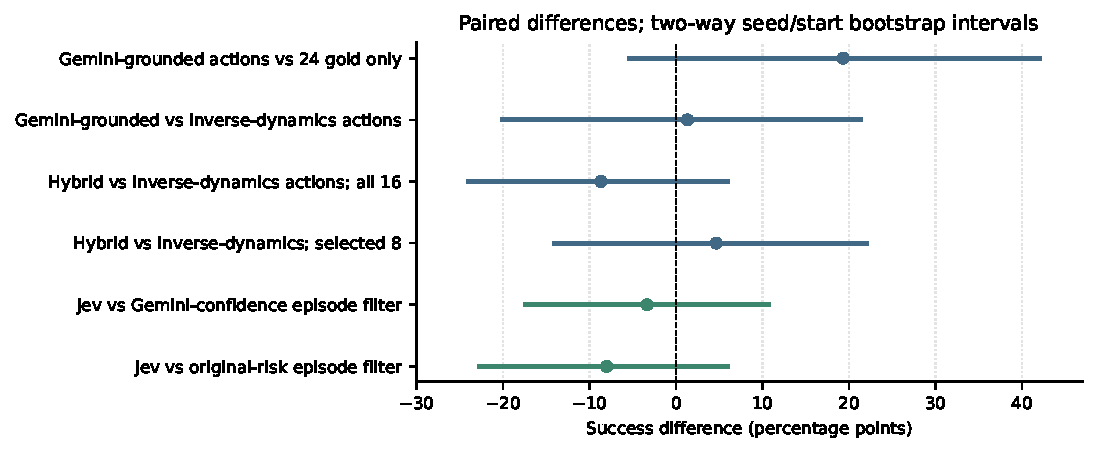
\includegraphics[width=\linewidth]{figs/policy_contrasts.pdf}
\caption{Selected paired success differences with two-way bootstrap
intervals resampling three policy seeds and 50 shared starts (10,000 draws,
fixed RNG seed 731). The first three contrasts were E3 primary comparisons;
the matched-filter E3 contrast is exploratory. The last two compare episode
selectors applied to identical saved hybrid actions, not different action
generators. Intervals describe this pilot and are not equivalence tests.}
\label{fig:contrasts}
\end{figure}

\section{Action and selection diagnostics}
Figure~\ref{fig:action} separates action reconstruction from policy utility.
On the 12-episode evaluation holdout, local B2 and B3 have position-action
mean absolute error (MAE) 0.1252 and 0.1197 in native normalized controller
units. Gemini's direct seven-value response has MAE 0.2411; its gripper
sign error is 0.3169, compared with 0.0949 for B2. Gemini semantics plus
local grounding have MAE 0.1323. State-only and shuffled-semantic controls
have 0.1372 and 0.1333. The 0.0010 real-versus-shuffled difference is
small; no paired episode-level interval is available in the saved summary,
so we make no content-specific gain claim. The hybrid MAE is 0.1308.
TypeSafe Jev has no action MAE because it never produced a seven-value
action. Its E3b role was selection.

\begin{figure}[t]
\centering
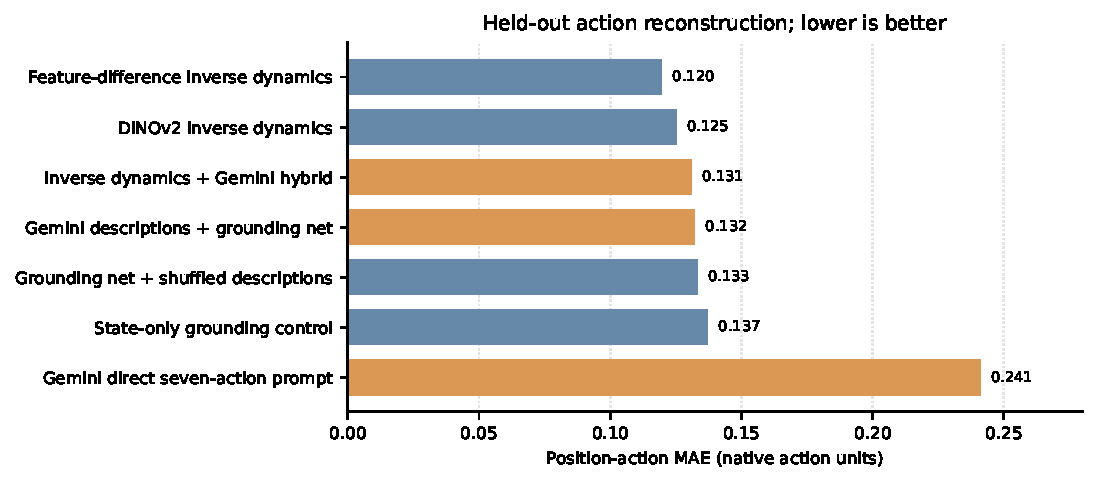
\includegraphics[width=\linewidth]{figs/action_error.pdf}
\caption{Action reconstruction on the 12-episode evaluation holdout.
Values are MAE in native action units, not percentages. These diagnostic
scores need not order policies by closed-loop success.}
\label{fig:action}
\end{figure}

E3's semantic probes improve on majority direction baselines for $y$
(0.691 versus 0.556) and $z$ (0.917 versus 0.793), but not $x$
(0.590 versus 0.657). Gripper-event probe accuracy equals the no-change
baseline (both 0.956). Thus the probes show some coarse signal, not
dependable contact understanding. The two-frame Gemini subset was collected
but not evaluated as a trained downstream policy ablation.

On the 527 E3b held-out transitions, the hybrid action's bad-event rate is
0.670. Hosted Jev's calibrated error-risk ranking has AUC 0.491 and Brier
score 0.239; the matched Gemini-confidence scores have 0.508 and 0.233;
the existing hybrid score has 0.680 and 0.214. The constant calibration
base-rate Brier is 0.233. Jev's Noul values are probabilities about the
worded ambiguity propositions, \emph{not} probabilities of motor error;
the isotonic map attempts that translation. Near-0.5 AUC means this chosen
hosted decision task provided no useful held-out error ranking here.
The E2 B2 risk map's held-out AUC was 0.695. Figure~\ref{fig:risk} shows
the E3b selection curves; scoring individual transitions for this diagnostic
differs from ranking whole episodes for policy training.

\begin{figure}[htbp]
\centering
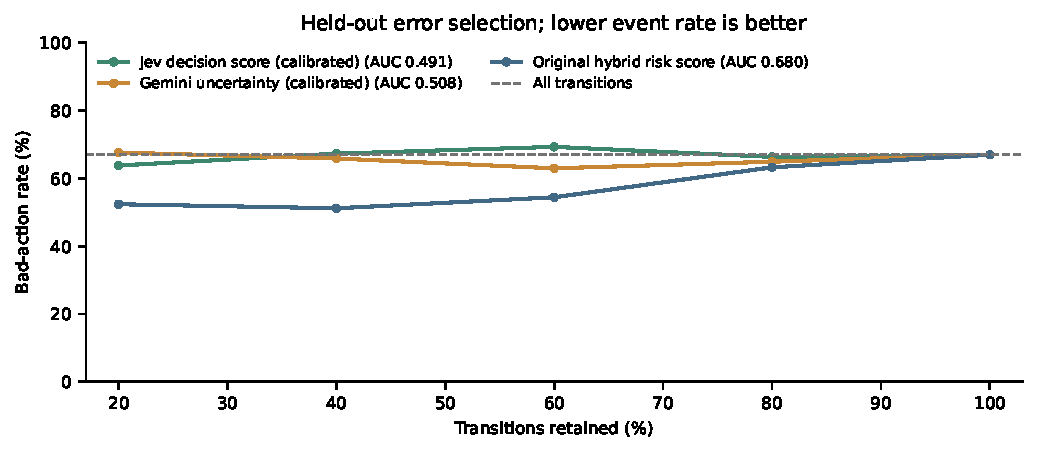
\includegraphics[width=0.82\linewidth]{figs/risk_coverage.pdf}
\caption{Bad-action rate as the lowest-risk fraction of held-out transitions
is retained. All three plotted scores refer to the same saved hybrid action
predictions. The old hybrid map is unchanged; the two new selectors use the
same tied-score-correct isotonic fit.}
\label{fig:risk}
\end{figure}

\section{Interpretation and limitations}
These experiments show that pseudo-action data can be useful in this Lift
setting; they do not isolate a necessary contribution from pretrained
semantics. Filtering can change training-set difficulty, number of examples,
and action-error distribution at once. Therefore a filtered policy's gain
cannot be attributed solely to better uncertainty calibration or to the
visual model. The historical filtering implementation has a tied-score
pooling defect in its isotonic helper. E3b used a corrected implementation
for \emph{both new selectors}; historical E3 results were preserved rather
than silently recomputed. Consequently hosted Jev versus Gemini confidence
is the cleaner comparison of new selectors.

The hosted study is particularly narrow. Jev read Gemini's already
compressed semantic JSON; it had no access to pixel evidence omitted or
misread by Gemini. Repeated descriptions collapse 1,646 transitions into 72
distinct hosted requests, restricting input diversity. Neither a result for
typed text decisions nor a result for one 24-label robot task measures
general hosted-Jev decision ability, direct visual control, cross-embodiment
transfer, or world-model prediction. E3b reused a pilot evaluation
population observed during E3. The 40-episode test remained locked;
three BC seeds and one visual/grounding seed limit generalization. No
methodological or statistical equivalence margin was prespecified.

The Gemini production pass also required documented integrity repairs.
After 539 legacy semantic cache entries, scene-specific episode XML was
restored before rendering; the old entries were excluded and the corrected
cache was rebuilt. Later action-alignment and CPU/MPS device fixes occurred
before the affected downstream results. These were repairs rather than
prespecified model improvements. The final E3 VLM summary counted only the
last resume pass (196 requests), not total campaign usage. Across cache
ledgers, 2,751 semantic, 1,646 direct, and 190 two-frame successful
annotations are covered. Cache tokens imply approximately \$26.23 at
listed Gemini prices; a read-only key query immediately after E3 showed
\$26.61 cumulative key usage including earlier invalidated calls, smoke
tests, and retries. E3b's TypeSafe decisions added \$0.00196014, with no
repeat Gemini calls. Billing uncertainty prevents assigning every cent of
the cumulative key amount to the final valid dataset.

\section{Related work and conclusion}
Latent action pretraining from unlabeled video followed by action adaptation
has established precedents: LAPA learns quantized latent actions before
VLA pretraining and robot-action fine-tuning \citep{lapa}; UniVLA learns
task-centric latents in DINO feature space with language context
\citep{univla}; and latent-action world models in the wild use constrained
continuous representations and action adapters \citep{wild}. CD-LAM studies
how irrelevant visual changes can contaminate learned action latents
\citep{cdlam}. Our single-task, small-budget pseudo-labeling and BC study
does not reproduce those systems, support a first-method claim, or make
cross-paper leaderboard comparisons.

The evidence supports a bounded conclusion: local inverse-dynamics
pseudo-labels improved Lift policy success over 24 gold demos. Gemini
semantics plus small grounding also improved the point estimate over 24
gold demos, but did not establish an advantage over B2. A later hosted
TypeSafe Jev decision layer did not improve selection of the saved hybrid
pseudo-actions over the matched Gemini-confidence control in this pilot.
The next decisive study should freeze a new contact-sensitive selector,
replicate across independent model-training seeds and a second task, and
evaluate on previously unseen episodes. Its advancement criterion should
require better calibrated held-out error ranking \emph{and} paired policy
utility above a matched local filtered baseline; failure on either rejects
that selector's claimed data-utility gain. A larger world-model claim
requires an actual action-conditioned world-model consumer.

\appendix
\section{Reproducibility and provenance}
The frozen configuration and implementation are in \path{config/},
\path{jev_research/}, and \path{research/jev/}. Lightweight run JSON and
paired rollout records used in this paper are committed under
\path{results/runs/}. Figure code is
\path{figs/make_policy_fig.py}; it reads those JSON files without
model inference. The E3b client and runner are
\path{research/jev/hosted_jev.py} and
\path{research/jev/run_hosted_jev.py}. Training/test access rules are
implemented in \path{jev_research/data.py} and
\path{jev_research/policy.py}. The dataset/controller audit is
\path{results/runs/lift_e0_none_seed0/e0_report.json}. E3b has 383 calibration
and 527 held-out transitions for the hybrid bad-event diagnostic. The
two-way intervals in Fig.~\ref{fig:contrasts} resample three policy-seed
indices and 50 shared start indices, with 10,000 draws and RNG seed 731.
This sensitivity analysis is descriptive, since three trained policies
cannot precisely identify between-seed variance.

\begin{thebibliography}{9}
\bibitem[Ye et al.(2025)]{lapa} S. Ye et al. Latent Action Pretraining from Videos.
ICLR, 2025. \url{https://arxiv.org/abs/2410.11758}.
\bibitem[Bu et al.(2025)]{univla} Q. Bu et al. UniVLA: Learning to Act Anywhere
with Task-centric Latent Actions. RSS, 2025.
\url{https://arxiv.org/abs/2505.06111}.
\bibitem[Garrido et al.(2026)]{wild} Q. Garrido et al. Learning Latent Action
World Models In The Wild. arXiv:2601.05230, 2026.
\url{https://arxiv.org/abs/2601.05230}.
\bibitem[Wei et al.(2026)]{cdlam} Y. Wei et al. Causally Debiased Latent
Action Model for Embodied Action Conditioned World Models.
arXiv:2607.09185, 2026. \url{https://arxiv.org/abs/2607.09185}.
\bibitem[TypeSafe AI(2026)]{typesafe} TypeSafe AI. System One documentation.
\url{https://docs.typesafe.ai/concepts/system-one}.
\bibitem[OpenRouter(2026)]{openrouter} OpenRouter. Submit a Decisions request.
\url{https://openrouter.ai/docs/api/api-reference/alphadecisions/submit-a-decisions-questions-and-answers-request}.
\end{thebibliography}
\end{document}
